\section{Evaluation}
~

\subsection{Environment setting}
~

The evaluation of the model is focused on two metrics : the makespan and the computing time once trained.
For the implementation of the model, python 3.10.12 with the PyTorch 2.4.1 library is used and runs on a google collab runtime
with 90 TPU cores.
The stochastic gradient descent is used for training with a learning rate of $0.001$ and a batch size of 250.

During the initial evaluation, an oversmoothing problem occured which lead to reducing the number of GCN layers to 1(see Section \ref{sec:model_design}).
Unfortunately reducing the number of GCN layers wasn't enough which lead 
to adding a regularization term to the loss function.
The idea is to tackle the over-smoothing probblem by forcing the model
to differentiate between the nodes' representation.
Hence, the regularization term is the squared inverse of the average euclidian distance 
between each of the nodes' latent representation, i.e., 
\begin{equation}
    \text{regTerm}(X) = \frac{1}{\sum_{i}\sum_{j > i} \Vert X_i - X_j\Vert_{2} }
\end{equation}
    
and the loss function then becomes
\begin{equation}
    loss(X, y) = \sum_{i} -y_i\log(x_i) + \text{regTerm}(X)
\end{equation}
with $x_i$ being the elements in $x$, the flattened matrix representation of $X$
and $y$ the true output (see Section \ref{sec:loss_design}).

\subsection{Dataset generation}
~

To generate the DAG tasks, the generator from \citet{zhao2020DAGsched} is used, which is also the one used in \citet{Lee2021GlobalDagSchedDRL}.
The random DAGs are generated using the following process :
The generator starts at a source node and expands outward, 
creating nodes in successive layers. The total number of layers, 
or maximum depth, is randomly determined to be between two values $a$ and $b$.
For each layer, the number of nodes generated is chosen uniformly, 
ranging from 2 up to the parallelism parameter, $p$ which in this case, 
is fixed at $p=8$. Nodes that do 
not already have connections can randomly connect to other nodes in 
the previous layer with a probability of $p_c=0.5$. After all layers 
are generated, any terminal nodes are linked to a final sink node. 
Both the source and sink nodes are used to structure the graph and 
have a fixed execution time of one unit each. Lastly, 
execution times are assigned randomly to all nodes while ensuring 
that the total workload sums up to $W = 1000$\cite{zhao2020DAGsched}.

To generate DAGs with a fixed number of nodes $n$, 
the generator is first used to generate 50000 DAG tasks
with different values for $a$ and $b$ depdending on what 
the value of $n$ is. Then, the generated DAGs with 
the specified number of nodes are retrieved from the dataset.
Specifically, Table \ref{tab:layer_num_minmax} 
shows the different $a$ and $b$ values according to $n$.

\begin{table}
    \centering
    \begin{tabular}{|c|c|c|}    
        \hline
        \textbf{n} & \textbf{a} & \textbf{b} \\
        \hline
        10 & 3 & 8 \\
        \hline
        \{20, 30\} & 5 & 8 \\
        \hline
        40 & 7 & 10 \\
        \hline
        50 & 10 & 15 \\
        \hline
    \end{tabular}
    \caption{dag generator $a$, minimum number of layers, and $b$, maximum
    number of layers, parameter values for generating 
    random DAGs according to number of fixed nodes per graph we need to retrieve afterwards.}
    \label{tab:layer_num_minmax}
\end{table}

Using those values, 1400 DAG tasks were retrieved and used for 
evaluation, for each value of $n$.
1000 of them were used for training the model, 400 for testing
and 100 of them were used to measure the computing time 
for both the ILP and the supervised ML methods.


\subsection{Computing time results}
~

The computing time for the ILP method is shown 
in Figure \ref{fig:ilp_compute_time}.
The ILP solver was timed out whenever the computing time exceeded 1 hour
and it did time out when considering systems of 2 and 4 cores, when the number of nodes
exceeded 20 nodes (i.e., 30, 40 and 50 nodes) per DAG task.
Hence, in the next sections, only 6 and 8 cores will be considered,
with the number of nodes not exceeding 30 nodes, to have enough
ILP solved DAGs for training the model. 

\begin{figure}
    \centering
    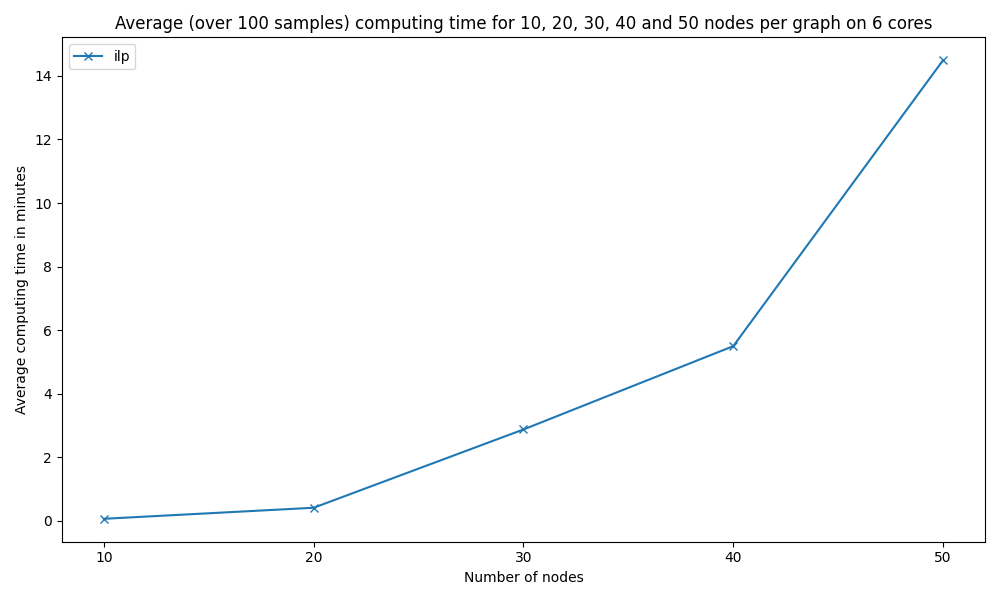
\includegraphics[width=\linewidth]{images/result_computing_time_ilp_m6.png}
    \caption{Average computing time for computing the optimal schedule
    of a single DAG task using the ILP method, in minutes, according to 
    the number of nodes in the DAG, on a system with 6 cores.}
    \label{fig:ilp_compute_time}
\end{figure}

As you can see from Figure \ref{fig:ilp_compute_time}, the more nodes there are on the system, 
the more time it takes for the ILP solver to compute the optimal schedule,
and it does so in, what it seems to be, an exponential growth.
Figure \ref{fig:ilp_compute_time} thus shows the non-scalability
of the ILP method, with the number of nodes per DAG increasing.

When comparing to the ML model's computing time (Figure \ref{fig:compute_time_ilp_model}),
you can see how 

\begin{figure}
    \centering
    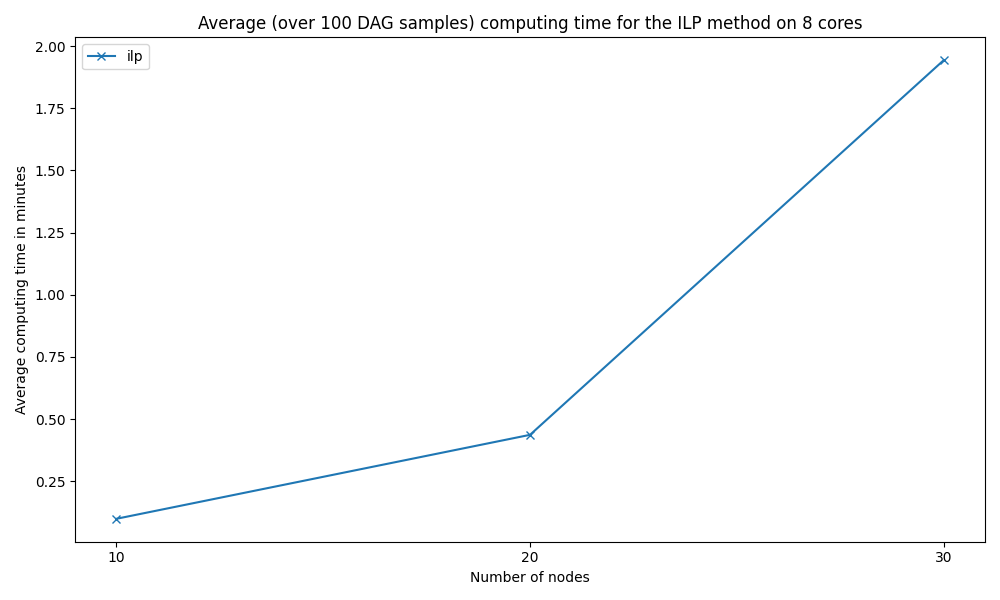
\includegraphics[width=\linewidth]{images/result_computing_time_ilp_m8.png}
    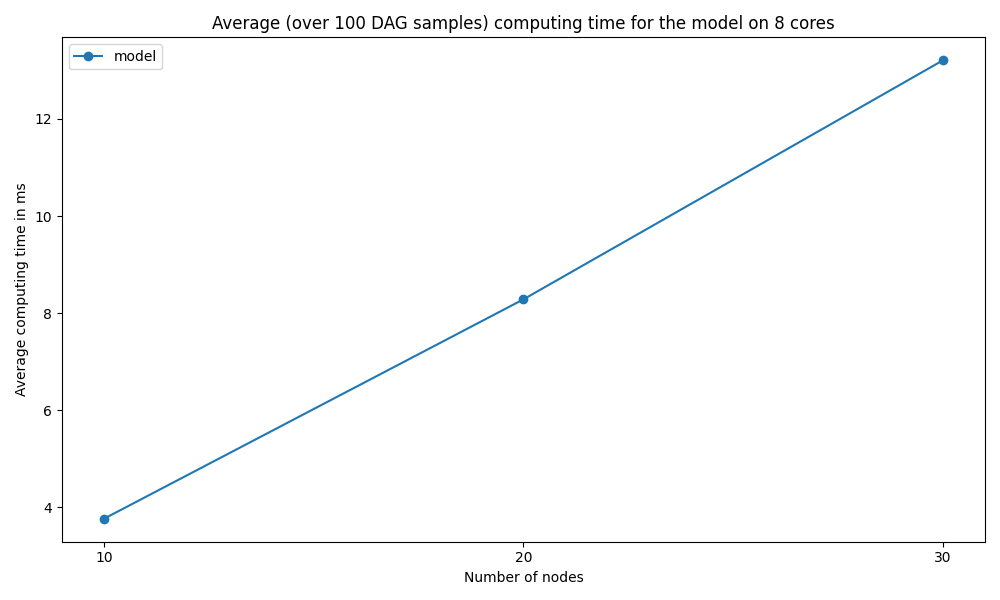
\includegraphics[width=\linewidth]{images/result_computing_time_model_m8.png}
    \caption{Average computing time for computing the optimal schedule
    of a single DAG task using the ILP method (top), in minutes,
    and using the ML model (bottom) according to 
    the number of nodes in the DAG, on a system with 8 cores.}
    \label{fig:compute_time_ilp_model}
\end{figure}